% Compile using: TEXINPUTS=minted/source: xelatex -shell-escape slides.tex
\documentclass[12pt,compress,english,utf8,t]{beamer}

\usepackage{etex}

\usepackage[english]{babel}

\usepackage{tikz}
\usepackage{booktabs}
\usepackage{ragged2e}

\makeatletter
\ifbeamer@draftmode
\usepackage{verbatim}
\newcommand{\inputminted}[2]{\verbatiminput{#2}}
\else
\usepackage{minted}
\setminted{linenos}
\fi
\makeatother

\usetikzlibrary{calc,shapes.callouts,shapes.arrows}
\definecolor{darkred}{RGB}{220,0,0}
\newcommand{\hcancel}[5]{%
    \tikz[baseline=(tocancel.base)]{
        \node[inner sep=0pt,outer sep=0pt] (tocancel) {#1};
        \draw[darkred, line width=1mm] ($(tocancel.south west)+(#2,#3)$) -- ($(tocancel.north east)+(#4,#5)$);
    }%
}%

\usepackage[protrusion=true,expansion=false]{microtype}

\usepackage{fontspec}
\newfontfamily\DejaSans{DejaVu Sans}

\title[Pugs, an experimental Perl 6 platform: a retrospective]{
  {\DejaSans ☺}
  A retrospective on Pugs
  {\DejaSans ☺}
}
\author[Augsburg.pm]{\texorpdfstring{
  \vspace{-0.5em} \\
  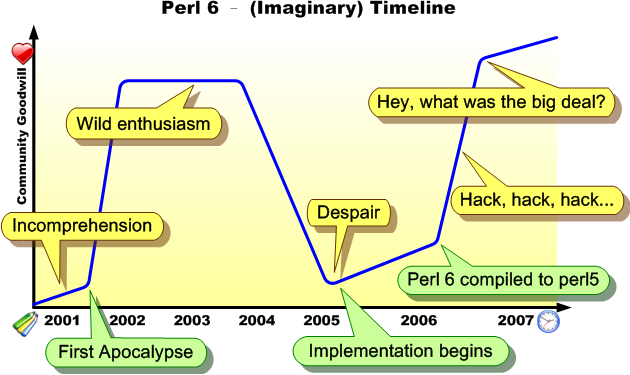
\includegraphics[scale=0.35]{images/timeline} \\[0.8em]
  Ingo Blechschmidt \\
  \scriptsize \texttt{<iblech@speicherleck.de>} \\
  April 13th, 2015
}{Ingo Blechschmidt}}
\date{April 13th, 2015}

\usetheme{Warsaw}
\usecolortheme{seahorse}
\definecolor{mypurple}{RGB}{60,0,255}  % Audrey's personal blog color, with full saturation
\setbeamercolor{structure}{fg=mypurple}
\usefonttheme{serif}
\usepackage{fontspec}
\defaultfontfeatures{Mapping=tex-text}
\setmainfont{Linux Libertine O}
\useinnertheme{rectangles}
\setbeamercovered{invisible}

\setbeamertemplate{title page}[default][colsep=-1bp,rounded=false,shadow=false]
\setbeamertemplate{frametitle}[default][colsep=-2bp,rounded=false,shadow=false,center]

\setbeamertemplate{navigation symbols}{}
\setbeamertemplate{headline}{}

\newcommand*\oldmacro{}%
\let\oldmacro\insertshorttitle%
\renewcommand*\insertshorttitle{%
  \oldmacro\hfill\insertframenumber\,/\,\inserttotalframenumber\hfill}

\newcommand{\hil}[1]{{\usebeamercolor[fg]{item}{\textbf{#1}}}}

\newcommand{\atpos}[1]{%
  \begin{tikzpicture}[remember picture, overlay]%
    \node[anchor=south east] at (current page.south east) {#1};
  \end{tikzpicture}%
}

\newcommand{\centeredpar}[2]{%
  \begin{center}
    \colorbox{white}{\parbox{#1\textwidth}{%
      #2%
    }}%
  \end{center}%
}

\newcommand{\sourcedquote}[4]{%
  ``#1''\par%
  {\raggedleft -- #2, #3, \href{#4}{\underline{link}}\par}%
}

% Gonzalo Medina, http://tex.stackexchange.com/a/228198
\makeatletter
\def\Mdescription#1{%
  \advance\beamer@descdefault by \labelsep%
  \list
  {}
  {\labelwidth\beamer@descdefault%
  \leftmargin\beamer@descdefault%
  \let\makelabel\beamer@descriptionitem
  \settowidth\labelwidth{\beamer@descriptionitem{#1}}%
  \setlength\leftmargin{\labelwidth}% 
  \addtolength\leftmargin{\labelsep}%
  }%
  \beamer@cramped%
  \raggedright
  \beamer@firstlineitemizeunskip%
}
\def\endMdescription{\ifhmode\unskip\fi\endlist}
\long\def\beamer@descriptionitem#1{%
  \def\insertdescriptionitem{#1}%
  {\usebeamertemplate**{description item}}\hfil}
\makeatother

\setbeameroption{show notes}
\setbeamertemplate{note page}[plain]

\begin{document}

\frame{\titlepage}

\frame[plain]{
  \centeredpar{0.9}{
    \justifying\scriptsize
    \textbf{Abstract.}
    ``Hi. Today I have started working on specifying and implementing
    Featherweight Perl 6 (FP6), a side-effect-free subset of Perl~6.''
    Audrey Tang used these words to unveil the Pugs project in February of 2005.
    Initially conceived as an implementation of a small subset of Perl~6 in
    Haskell, the project quickly grew to contain a full-fledged compiler and
    interpreter for Perl~6 and attracted a large and diverse community.

    \medskip
    The talk will give a subjective survey of the history of Pugs. We will pay
    particular attention to the special manner with which Audrey Tang led the project and
    what the philosophy ``-O\emph{fun}'' meant to the developers. We'll also discuss
    which parts of Pugs were absorbed into other implementations of Perl~6 and
    which influence Pugs had on the Perl and Haskell communities.
    \medskip

    \textbf{About me.} While a school student, I contributed to Pugs in
    2005, at first by porting modules and writing tests, then gradually also by
    writing Haskell code and later by implementing a JavaScript backend. Audrey
    and the unique spirit in the Pugs community had a strong and lasting
    influence on me (exposing me to Haskell, category theory, and
    a beautiful way of tending communities); I look back on very exciting and
    fun days.
    \medskip

    \textbf{Warning.} The account is mostly from memory and not properly
    researched. Try not to trust it! Also note that the timeline covers only
    the year 2005 and that \emph{the code excerpts are
    edited for legibility}, i.\,e.\@ shortened at a few places and not
    reproduced verbatim.
    \par
  }
}

\setcounter{tocdepth}{2}
\frame{\tableofcontents}

\section{A glimpse of Perl 6}

\begin{frame}[fragile]\frametitle{A glimpse of Perl 6}
  \only<1>{\inputminted{perl}{code-snippets/a-glimpse-of-perl6-1.pl}}
  \only<2>{\inputminted{perl}{code-snippets/a-glimpse-of-perl6-2.pl}}
  \pause
  \pause

  \justifying
  closures \textbullet{}
  anonymous types \textbullet{}
  roles and traits \textbullet{}
  named arguments \textbullet{}
  expressive routine signatures \textbullet{}
  a strong meta object system \textbullet{}
  macros \textbullet{}
  state variables \textbullet{}
  named regexes for easy reuse \textbullet{}
  cleaned up regular expressions \textbullet{}
  grammars for parsing \textbullet{}
  lazy lists \textbullet{}
  junctions of values \textbullet{}
  optional type annotations (gradual typing) \textbullet{}
  powerful run-time multi dispatch \textbullet{}
  lexical imports
  \par
\end{frame}

\begin{frame}
  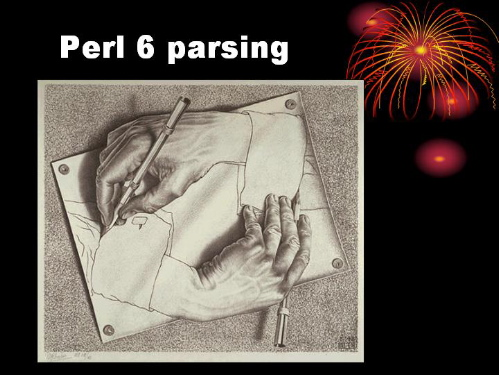
\includegraphics[width=0.45\textwidth]{images/perl-6-parsing.jpeg}

  \hfill
\includegraphics[width=0.45\textwidth]{images/implementing-perl-6.jpeg}
\end{frame}

\section{Timeline of Pugs development}

\subsection{The beginning}

\logo{
\includegraphics[scale=0.13]{images/audreyt2.jpeg}}
\begin{frame}\frametitle{The beginning}
  \vspace*{-1em}
  \centeredpar{0.9}{
    \hil{``Hi. Today I have started working on specifying and implementing
    Featherweight Perl 6 (FP6), a side-effect-free subset of Perl~6.''}

    \raggedleft -- Audrey Tang, February 2nd, 2005
  }

  \begin{Mdescription}{2001}
    \item[2001] Apocalypse 1, first Perl 6 design document
    \item[2004] Many Apocalypse and Synopse documents
    \item[2005] Active discussion on perl6-language@perl.org
    \item[2005] Pugs, providing the first usable implementation
    \item[]
    \item[2005] Facebook
    \item[2005] YouTube
    \item[2008] GitHub
  \end{Mdescription}
\end{frame}
\logo{}

\begin{frame}\frametitle{Haskell?}
  \begin{center}
    \vbox{
\includegraphics[width=0.35\textwidth]{images/haskell-meme-2.jpeg}
\includegraphics[width=0.35\textwidth]{images/haskell-meme-4.jpeg}\\
    
\includegraphics[width=0.35\textwidth]{images/haskell-meme-5.jpeg}
\includegraphics[width=0.35\textwidth]{images/haskell-meme-6.jpeg}}
  \end{center}
\end{frame}

% http://wayback.archive.org/web/20050209100505/http://haskell.org/hawiki/Perl6UsersGolfingSystem
\begin{frame}[fragile]\frametitle{Screenshot}\scriptsize
  \vspace{-2.0em}
  \begin{verbatim}.=====. __  __  ____   ___    _________________________________________
||   || ||  || ||  || ||__'   Pugs 6: Based on the Perl 6 Synopses
||====' ||__|| ||__||  __||   Copyright (c) 2005 Autrijus Tang
||      `===='  ___|| `==='   World Wide Web: http://autrijus.org/pugs
||             `===='         Report bugs to: autrijus@autrijus.org
==           Version: 6.0.0   =========================================

Welcome to Pugs -- Perl6 User's Golfing System
Type :h for help

pugs> :h
Commands available from the prompt:
:h              = show this help message
:q              = quit
. <exp>         = show the syntax tree of an expression
? <exp>         = evaluate an expression

pugs> . ('1' & "2") * (3.0 | "4abcd")
Op2 "*" (Op2 "&" (Val (VStr "1")) (Val (VStr "2"))) (Op2 "|" (Val (VNum 3.0)) (Val (VStr "4abcd")))

pugs> ('1' & "2") * (3.0 | "4abcd")
((3.0 | 4.0) & (6.0 | 8.0))

pugs> :q
Leaving pugs.\end{verbatim}
\end{frame}

\note{
  \begin{itemize}
    \justifying
    \item \sourcedquote{As I'm finding my way through TaPL and ATTaPL today, it occurs to me that
    I should implement a real language as an exercise; that real language turns
    out to be Perl~6. So it begins \ldots}{Audrey Tang}{February 1st,
    2005}{http://wayback.archive.org/web/20050206202119/http://use.perl.org/~autrijus/journal/}
    \item TaPL refers to \emph{Types and Programming Languages}, a
    computer-science book on implementing programming languages.
    \item Audrey quickly dropped her initial plan to focus on a
    side-effect-free subset.
    \item There was an implementation before Pugs, a tiny
    project sitting in the Parrot source tree.
    \item Audrey's first post contained a language semantics question. This
    would be the beginning of continuing refinements of the specification, made
    possible by the existence of a useful Perl~6 platform which allowed people
    to play with Perl~6.
  \end{itemize}
}

\note{
  \begin{itemize}
    \justifying
    \item \sourcedquote{This last year, we were starting to lose our sense of
    fun in the Perl community. Though we tried to be careful about not making
    promises, everyone knew in their hearts that five years is an awfully long
    time to wait for anything. People were getting tired and discouraged and a
    little bit dreary.

    Then [Audrey Tang] showed up.}{Larry Wall}{August
    2005 (OSCON)}{http://www.perl.com/pub/2005/09/22/onion.html}
  \end{itemize}
}


\subsection{The early days}

\begin{frame}[label=the-early-days]\frametitle{The early days}
  \begin{Mdescription}{Day 00}
    \item[Day 4] ``Parsec; 90\,\% of operators implemented!''
    \hfill\hyperlink{parsec}{\beamerbutton{see code}}
    \item[Day 8] ``Pugs 6.0.2; Turing Completeness''
    \hfill\hyperlink{turing-completeness}{\beamerbutton{see code}}
    \item[Day 12] ``Refactoring''
    \hfill\hyperlink{refactoring}{\beamerbutton{see code}}
    \item[Day 13] ``Continuations''
    \hfill\hyperlink{continuations}{\beamerbutton{see code}}
    \item[Day 14] ``All tests successful''
    \hfill\hyperlink{all-tests-successful}{\beamerbutton{see code}}
    \item[Day 20] ``6.0.8''
    \hfill\hyperlink{608}{\beamerbutton{see code}}
    \item[Day 23] ``Test.pm flies!''
    \hfill\hyperlink{testpm}{\beamerbutton{see code}}
  \end{Mdescription}

  \hyperlink{further-highlights}{\beamerbutton{skip details}}
\end{frame}

\note{
  \justifying
  As can be seen by the journal headlines, Pugs was extremely fast-moving. In
  the early days, a Pugs build of a day ago was considered to be vastly
  outdated. This had two reasons:
  \begin{itemize}
    \justifying
    \item Firstly, Audrey was an astoundingly productive hacker, rapidly
    implementing major features and attracting a large community of fellow
    \emph{lambdacamels}.
    \item Secondly, Haskell's unique features made it the language of choice
    for implementing Perl~6. It allowed both for quick prototyping and easy
    refactoring.
  \end{itemize}
}

\logo{\hyperlink{the-early-days}{\beamerbutton{Continue slides \ldots}}}

\begin{frame}[label=parsec]\frametitle{Day 4: ``Parsec; 90\,\% of operators implemented!''}
  % https://github.com/audreyt/pugs/blob/e760c8600350603c10c825caf17ca5ce1e2846ae/src/Parser.hs
  % https://github.com/audreyt/pugs/blob/e760c8600350603c10c825caf17ca5ce1e2846ae/src/Prim.hs
  \only<1>{
    \inputminted{haskell}{code-snippets/day4-ast.hs}
  }
  \pause

  \inputminted{haskell}{code-snippets/day4-parser.hs}
  \medskip
  \inputminted{haskell}{code-snippets/day4-prim.hs}
\end{frame}

\begin{frame}[label=turing-completeness]\frametitle{Day 8: ``Pugs 6.0.2; Turing Completeness''}
  % https://github.com/audreyt/pugs/blob/e760c8600350603c10c825caf17ca5ce1e2846ae/src/Eval.hs
  User-defined subroutines, variable binding, \ldots\par
  \inputminted{haskell}{code-snippets/day8-eval.hs}
\end{frame}

\begin{frame}[label=refactoring]\frametitle{Day 12: ``Refactoring''}
  eval(), rand(), \ldots\par
  \inputminted{haskell}{code-snippets/day12-prim.hs}
\end{frame}

\begin{frame}[label=continuations]\frametitle{Day 13: ``Continuations''}
  \inputminted{haskell}{code-snippets/day13-monads.hs}
  \bigskip
  \inputminted{haskell}{code-snippets/day13-ast.hs}
\end{frame}

\begin{frame}[label=all-tests-successful]\frametitle{Day 14: ``All tests successful''}
  \inputminted{perl}{code-snippets/day14-basic.pl}
\end{frame}

\begin{frame}[label=608]\frametitle{Day 20: ``6.0.8''}
  Hashes, pairs, many IO primitives, \ldots\par
  \inputminted{perl}{code-snippets/day20-ycombinator.pl}
\end{frame}

\begin{frame}[label=testpm]\frametitle{Day 23: ``Test.pm flies!''}
  First Perl 6 module, more than 400 unit tests, \ldots\par
  \inputminted{perl}{code-snippets/day23-test.pm}
\end{frame}


\subsection{Further highlights}

\logo{}
\begin{frame}[label=further-highlights]\frametitle{Further highlights}
  \begin{Mdescription}{Day 000}
    \item[Day 47] ``Perl 5 regular expressions landed.''
    \hfill\hyperlink{perl5re}{\beamerbutton{see code}}

    \item[Day 50] Compiling to Parrot

    \item[Day 69] Autovivification, tied magic, slice assignment
    \hfill\hyperlink{tied-env}{\beamerbutton{see code}}

    \item[Day 85] BEGIN blocks
    \hfill\hyperlink{begin-blocks}{\beamerbutton{see code}}

    \item[Day 87] ``STM: Atomic power!''
    \hfill\hyperlink{stm}{\beamerbutton{see code}}

    \item[Day 88] ``A shiny new monad.''
    \hfill\hyperlink{shiny-monad}{\beamerbutton{see code}}

    \item[Day 99] ``Full named rules!''
    \hfill\hyperlink{rules}{\beamerbutton{see code}}

    \item[Day 100] ``OO support landed!'' (a first sketch)

    \item[Day 107] User-defined operators, Inline::Pugs
    \hfill\hyperlink{user-defined-ops}{\beamerbutton{see code}}

    \item[Day 109] gather/take
    \hfill\hyperlink{gather-take}{\beamerbutton{see code}}

    \item[Day 111] Hyper operators
    \hfill\hyperlink{hyper-operators}{\beamerbutton{see code}}

    \item[Day 113] ``Pugs runs CPAN modules!''
    \hfill\hyperlink{pugs-cpan}{\beamerbutton{see code}}
  \end{Mdescription}
\end{frame}

\begin{frame}[label=further-highlights-cont]\frametitle{Further highlights, cont'd}
  \begin{Mdescription}{Day 000}
    \item[Day 117] evalbot (using a new safe mode)

    \item[Day 128] Academic paper for the Haskell Workshop 2005
    (rejected)

    \item[Day 162] ``Say hello to P5ugs!''

    \item[Day 164] ``Perl 6 compiled to\ldots{} JavaScript!''
    \hfill\hyperlink{pil2js}{\beamerbutton{see code}}
    \item[Day 166] ``Mandel.p6 on JavaScript.''
    \item[Day 177] ``JS backend 43\% pass''
    \item[Day 193] ``JSAN and CPAN, here we come!''
    \item[Day 219] Perl 6 on JavaScript passes 91\%.
  \end{Mdescription}

  \hyperlink{the-end}{\beamerbutton{skip details}}
\end{frame}
% Finished http://pugs.blogs.com/pugs/2005/12/page/1/.

% Day 162: Say hello to P5ugs!
% `mandel.p6` compiled to Parrot: Mar 24

% XXX: Perl-6-on-Perl-5 effort

\logo{\hyperlink{further-highlights}{\beamerbutton{Continue slides \ldots}}}

\subsubsection{Day 47: ``Perl 5 regular expressions landed.''}

\begin{frame}[label=perl5re]\frametitle{Day 47: ``Perl 5 regular expressions landed.''}
  \inputminted{text}{code-snippets/day47-regex.pl}
\end{frame}


\subsubsection{Day 69: Tied \texttt{\%*ENV}}

\begin{frame}[label=tied-env]\frametitle{Day 69: Tied \texttt{\%*ENV}}
  \inputminted{haskell}{code-snippets/day69-ast.hs}
\end{frame}


\subsubsection{Day 85: BEGIN blocks}

\begin{frame}[label=begin-blocks]\frametitle{Day 85: BEGIN blocks}
  \inputminted{haskell}{code-snippets/day85-parser.hs}
\end{frame}


\subsubsection{Day 87: ``STM: Atomic power!''}

\begin{frame}[label=stm]\frametitle{Day 87: ``STM: Atomic power!''}
  \inputminted{perl}{code-snippets/day87-atomic.pl}
\end{frame}


\subsubsection{Day 88: ``A shiny new monad.''}

\begin{frame}[label=shiny-monad]\frametitle{Day 88: ``A shiny new monad.''}
  % http://pugs.blogs.com/pugs/2005/04/day_88_a_shiny_.html

  \begin{tabbing}
    \hil{$\langle$audreyt$\rangle$} \= \kill
    \hil{$\langle$obra$\rangle$} \> What the hell changed in the last 12 hours with pugs? \\[0.3em]
    \hil{$\langle$obra$\rangle$} \> I mean it smoked 30\,\% faster. \\[0.3em]
    \hil{$\langle$audreyt$\rangle$} \> oh. yeah. I rewrote the monad
  \end{tabbing}
\end{frame}


\subsubsection{Day 99: ``Full named rules!''}

\begin{frame}[label=rules]\frametitle{Day 99: ``Full named rules!''}
  % http://pugs.blogs.com/pugs/2005/05/day_99_full_nam.html

  Perl 6 rules: Named regexes that form a formal grammar. Capture objects can
  be full-fledged abstract syntax trees.

  % http://perlgeek.de/en/article/mutable-grammar-for-perl-6 (2008)
  \inputminted{perl}{code-snippets/day99-rules.pl}
\end{frame}


\subsubsection{Day 107: User-defined operators}

\begin{frame}[label=user-defined-ops]\frametitle{Day 107: User-defined operators}
  % http://pugs.blogs.com/pugs/2005/05/day_106_apacher.html

  \inputminted{perl}{code-snippets/day107-user-defined-ops.pl}
  \medskip
  \inputminted{haskell}{code-snippets/day107-parser.hs}
\end{frame}


\subsubsection{Day 109: gather/take}

\begin{frame}[label=gather-take]\frametitle{Day 109: gather/take}
  % http://pugs.blogs.com/pugs/2005/05/day_109_corouti.html

  \vspace{-0.5em}
  \only<1>{\inputminted{perl}{code-snippets/day109-gather-take.pl}}

  \pause
  \inputminted{haskell}{code-snippets/day109-prim.hs}

  \vspace{-4em}
  \begin{columns}
    \begin{column}{0.7\textwidth}
    \end{column}
    \begin{column}{0.3\textwidth}
      \scriptsize
      \inputminted[linenos=false]{perl}{code-snippets/day109-gather-take.pl}
    \end{column}
  \end{columns}
\end{frame}


\subsubsection{Day 111: Hyper operators}

\begin{frame}[label=hyper-operators]\frametitle{Day 109: Hyper operators}
  % http://pugs.blogs.com/pugs/2005/05/day_111_hyper_o.html

  \inputminted{perl}{code-snippets/day111-hyper-operators.pl}
\end{frame}


\subsubsection{Day 113: ``Pugs runs CPAN modules!!''}

\begin{frame}[label=pugs-cpan]\frametitle{Day 113: ``Pugs runs CPAN
modules!!''}
  % http://pugs.blogs.com/pugs/2005/05/day_113_pugs_ru.html

  \inputminted{perl}{code-snippets/day113-pugs-cpan.pl}
\end{frame}

\subsubsection{Day 164 and others: Perl 6 on JavaScript}
\logo{\hyperlink{further-highlights-cont}{\beamerbutton{Continue slides \ldots}}}
\begin{frame}[label=pil2js]\frametitle{Day 164 and others: Perl 6 on JavaScript}
  \begin{center}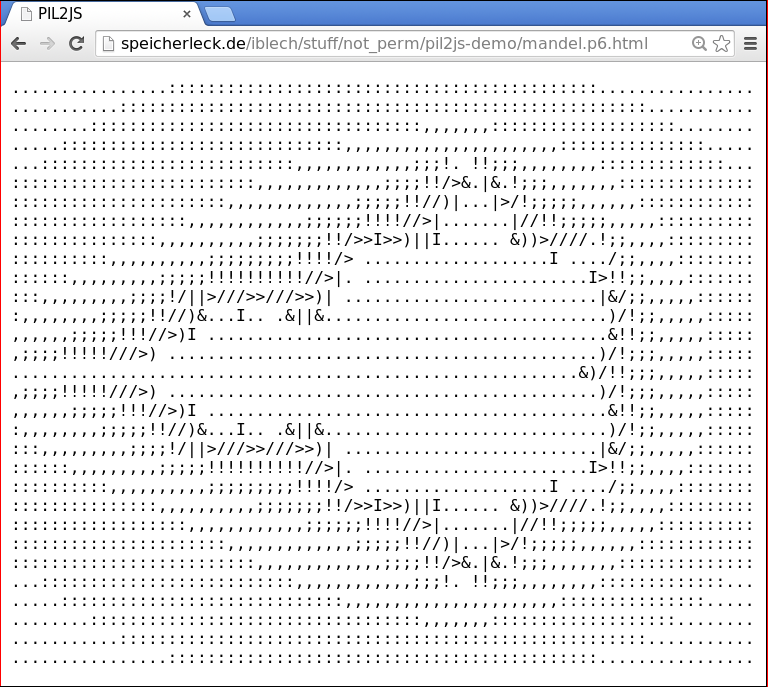
\includegraphics[scale=0.25]{images/mandel-in-the-browser}\end{center}

  \inputminted{perl}{code-snippets/day193-jsan.pl}
\end{frame}
% http://irclog.perlgeek.de/perl6/2005-07-17

\note{
  \begin{itemize}
    \justifying
    \item JSAN was an attempt to bring a CPAN-like platform to JavaScript. The
    JavaScript backend was able to use JSAN modules.
    \item Foreshadowing node.js:
    \sourcedquote{It is entirely possible that the JavaScript backend may prove
    to be the most important one. [\ldots]
    Indeed, if JavaScript2 does survive the standardization
    process, it is entirely possible that it may become the next Ruby, because
    writing programs that run at both client and server side is a strong
    motivation -- the same reason to keep Pugs targetable to multiple
    backends.}{Audrey Tang}{October 30th,
    2005}{http://wayback.archive.org/web/20060924085336/http://use.perl.org/journal.pl?op=display&uid=1505&start=10}
  \end{itemize}
}

% XXX: Hackatons
% Vienna?
% Leo in June 2005
% Toronto in June 2005
% Liz in October 2005

\logo{}

\subsection{The end}

\begin{frame}[label=the-end]\frametitle{The end}
  \begin{Mdescription}{Beginning of 2007}
    \item[Beginning of 2007]
      Active development of Pugs stalls.
  \end{Mdescription}

  \begin{center}
    \emph{-- discussion only verbally --}
  \end{center}
\end{frame}

\note{
  \begin{itemize}
    \justifying
    \item For school reasons, I withdrew from Pugs development before its active phase
    ended. Therefore I'm not qualified to report on the reasons for its end
    and deem it unresponsible to speculate in public.
    \item Note that Pugs is still kept compatible with respect to new GHC
    releases.
  \end{itemize}
}

% Reasons may or may not include (sorted alphabetically):
%
% * "Low-hanging fruits" gradually vanished. Progress was not as rapid as
%   in the early days.
%
% * Audrey got ill.
%
% * Efforts were redirected to bringing some of Perl 6's unique features
%   to Perl 5.
%
% * Further development required advances in the host language, Haskell.
%
% * Missed insight: A Perl 6 compiler has to be tightly coupled with a
%   rules engine, to allow for the compile-time syntax modifications
%   which Perl 6 allows.
%
% Also see the thread http://perlmonks.org/?node_id=835731, containing posts
% from chromatic and Audrey. *Please* don't trust my assessment. I don't have
% any personal familiarity with the end of Pugs's active life and gathered
% those speculations only from various online sources.


\section{Pugs's unique culture}

% XXX: Academic paper-reading

\subsection{Test-driven development}

\begin{frame}\frametitle{Test-driven development}
  \begin{itemize}
    \item Tests as to do lists.
    \item Tests as bug reports.
    \item Tests as specification.
  \end{itemize}

  \begin{center}
    
\includegraphics[scale=0.5]{images/test-all-the-things.jpeg}
  \end{center}
\end{frame}


\subsection{Transparency}

{\setbeamertemplate{background canvas}{
\includegraphics[width=\paperwidth]{images/transparency}}
\begin{frame}\frametitle{Transparency}
  \begin{itemize}
    \item Audrey's journal: \\
    \qquad\quad documenting progress, \\
    \qquad\quad\qquad\quad spreading excitement
    \item Public IRC logs
    \item svnbot, announcing new commits
    \item ``Private code $=$ dead code.'' ``url?''
  \end{itemize}
\end{frame}}


\subsection{Optimizing for fun}

\begin{frame}\frametitle{Pugs's unique culture}
  \begin{center}
    \Huge
    \only<1>{\hcancel{\scalebox{2.5}{-O\hil{2}?}}{0pt}{3pt}{0pt}{-2pt}}
    \only<2>{\hcancel{\scalebox{2.5}{-O\hil{s}?}}{0pt}{3pt}{0pt}{-2pt}}
  \end{center}
\end{frame}

{\setbeamercolor{frametitle}{bg=mypurple,fg=white}
\setbeamertemplate{background canvas}{
\includegraphics[width=\paperwidth]{images/mario.jpeg}}
\begin{frame}\frametitle{Optimizing for fun}
  \begin{center}
    \Huge
    \scalebox{2.5}{-O\hil{fun}!}
  \end{center}

  \begin{itemize}
    \item Liberal granting of commit bits.
    \item Forgiveness $>$ permission.
    \item ``Imagineering'', sketching ideas with code.
    \item Many subprojects, avoiding deadlocks.
  \end{itemize}

  \pause
  \centeredpar{0.85}{
    \hil{Audrey single-handedly bootstrapped a diverse and tight-knit
    community of lambdacamels, sharing a common vision and thoroughly
    enjoying their time.}
    Thank you, Audrey. $\heartsuit$
  }
\end{frame}}

\note{
  \begin{itemize}
    \justifying
    \item ``Patches are boring, commits are fun.''
    \item The diverse community was very welcoming. Trolls were hugged and
    turned into committers.
    \item Somebody would come to \#perl6 and mention that \$FEATURE
    does not work yet. Audrey would send them a commit bit, ask to create a
    test exemplifying the missing feature, and often implement the feature till
    the next day (or hour (or quarter of an hour)).
    \item People worked on the Haskell parts of the interpreter and the
    compiler, on unit tests, on porting and creating modules, on examples and
    documentation, on various backends (Perl~5 and JavaScript) written in
    Perl~5, on fun side projects (such as understanding type inference
    algorithms), and many other things.
    \item
    \href{https://speakerdeck.com/audreyt/ofun-optimizing-for-fun}{Audrey's
    slides \emph{-Ofun: Optimizing for Fun}} and Geoff Broadwell's
    \href{https://web.archive.org/web/20051125071047/http://www.oreillynet.com/pub/wlg/7996}{article
    on O'Reilly Network} are highly recommended reading.
  \end{itemize}
}

\note{
  \begin{itemize}
    \justifying
    \item \sourcedquote{One of my goals of this project is to keep it dual-cultured. So the
    source tree is managed with both svk and darcs; the build system requires
    both Perl5 and GHC; I will submit my Apocrypha series of design documents
    as monthly articles to both Perl.com and The Monad Reader; the project info
    is on both CPAN and the Haskell Wiki; etc, etc.}{Audrey Tang}{February 6st,
    2005}{http://wayback.archive.org/web/20050206202119/http://use.perl.org/~autrijus/journal/}

    \item \sourcedquote{In other news, Pugs was mentioned on The Haskell
    Sequence today. Indeed, I have noted that a significant part of questions
    asked in \#haskell are from camelfolks. Conversely, we saw a large influx
    from lambdafolks to \#perl6 as well. Lots of knowledge transfer is
    happening, which makes me really happy.}{Audrey Tang}{February 24th,
    2005}{http://pugs.blogs.com/pugs/2005/02/day_24_an_amazi.html}
  \end{itemize}
}


\section{Lasting contributions of Pugs}

\begin{frame}\frametitle{Lasting contributions of Pugs}
  \begin{itemize}
    \item Renewed interest in Perl 6.
    \item Major refinements of the specification.
    \pause
    \item \hil{The test suite.} Approximately 20\,000 unit tests.
    \pause
    \item The culture.
    \item Publicity for Haskell.
    \pause
    \item \hil{Moose.}

    \begin{center}
\includegraphics[scale=0.3]{images/moose.jpeg}\end{center}
  \end{itemize}
\end{frame}

\note{
  \begin{tabbing}
    \hil{$\langle$stevan$\rangle$} \= \kill
    \#perl6 on 2005-07-20: \\
    \hil{$\langle$stevan$\rangle$} \>
    geoffb: I think ``moose'' is a private joke between nothingmuch \\
    \> and himself :) \\\\
    \#perl6 on 2006-03-06: \\
    \hil{$\langle$stevan$\rangle$} \>
    audreyt: I have to run (dinnertime), but I have to show you \\
    \> Moose.pm soon, it is my (Class::MOP based) answer to Spiffy :)
  \end{tabbing}

  \justifying
  stevan is, of course, Stevan Little. Moose originated in Stevan's work 
  on the Perl 6 metamodel (which governs objects, classes, and metaclasses).
  \par
}

\note{
  \justifying\scriptsize
  \sourcedquote{It came out of the Pugs project, which is a project that in
  about 2005 started. It was Audrey Tang who was had decided that she wanted to
  implement Perl 6 in Haskell. So it was sort of a very fun project. Audrey
  coined the term “O-fun,” optimized for fun.\medskip

  And lot of the goal of the project was to get some juice flowing back into
  the Perl 6 community and really get a working or a semi-working
  implementation so people could play with it.\medskip

  One of the things that I did in that project was to prototype the object
  system for Perl 6. I read over the Apocalypse 12, read up on a number of
  different object systems in different languages such as Smalltalk, CLOS,
  which is the Common Lisp Object System. Objective fees, objects run time,
  Ruby, Python, all those things. We were doing a lot of research at time and
  we tried to put a lot of that stuff, a lot of the good ideas, into the Perl 6
  object system.\medskip

  And then basically as the Pugs project started to peter out, I found myself
  going back to my work code, which was your basic vanilla Perl 5.OO. And I
  really craved all the features that I had been prototyping.\medskip

  So months here and months there, I fiddled around and I finally came up with
  a module called Class::MOP which is basically the basis on which Moose sits.
  And so a couple months after Class::MOP, we released Moose and sort of got
  running from there.}{Stevan Little}{December
  2010}{http://perlcast.com/2010/07/12/stevan-little-on-moose/}
}

\appendix


\end{document}

http://www.slideshare.net/autang/pugs-a-perl-6-implementation
http://www.slideshare.net/autang/ofun-optimizing-for-fun
http://perlmonks.org/?node_id=835731

https://gist.github.com/quchen/5280339
trolling #haskell

http://developers.slashdot.org/story/05/10/09/1831219/optimizing-development-for-fun
frivolous toy interpreter

http://www.nntp.perl.org/group/perl.perl6.language/2005/02/msg19263.html
kudos to autrijus

pioneering techniques:
GADTs

fun:
slides "Perl 6, genau jetzt!"

porting modules
testing stuff
force_todo
some builtins
IRC library and bots
hyper operators
state/FIRST
macros
smokeserver
PIL2JS

http://pugs.blogs.com/pugs/2005/05/day_109_corouti.html
<iblech> Yeah, I start to grok Haskell :)
<autrijus> iblech++ # demonstrating that the productivity is really not me,
it's really Haskell :)

http://perlmonks.org/?node=perl+oddities

http://strangelyconsistent.org/blog/happy-10th-anniversary-perl-6
https://www.fsf.org/blogs/community/recognizing-an-inspiring-woman-for-ada-lovelace-day-audrey-tang
